\documentclass[]{article}
\usepackage{lmodern}
\usepackage{amssymb,amsmath}
\usepackage{ifxetex,ifluatex}
\usepackage{fixltx2e} % provides \textsubscript
\ifnum 0\ifxetex 1\fi\ifluatex 1\fi=0 % if pdftex
  \usepackage[T1]{fontenc}
  \usepackage[utf8]{inputenc}
\else % if luatex or xelatex
  \ifxetex
    \usepackage{mathspec}
  \else
    \usepackage{fontspec}
  \fi
  \defaultfontfeatures{Ligatures=TeX,Scale=MatchLowercase}
\fi
% use upquote if available, for straight quotes in verbatim environments
\IfFileExists{upquote.sty}{\usepackage{upquote}}{}
% use microtype if available
\IfFileExists{microtype.sty}{%
\usepackage{microtype}
\UseMicrotypeSet[protrusion]{basicmath} % disable protrusion for tt fonts
}{}
\usepackage[margin=1in]{geometry}
\usepackage{hyperref}
\hypersetup{unicode=true,
            pdftitle={Méthodes de Monte Carlo},
            pdfauthor={Pierre Gloaguen},
            pdfborder={0 0 0},
            breaklinks=true}
\urlstyle{same}  % don't use monospace font for urls
\usepackage{graphicx,grffile}
\makeatletter
\def\maxwidth{\ifdim\Gin@nat@width>\linewidth\linewidth\else\Gin@nat@width\fi}
\def\maxheight{\ifdim\Gin@nat@height>\textheight\textheight\else\Gin@nat@height\fi}
\makeatother
% Scale images if necessary, so that they will not overflow the page
% margins by default, and it is still possible to overwrite the defaults
% using explicit options in \includegraphics[width, height, ...]{}
\setkeys{Gin}{width=\maxwidth,height=\maxheight,keepaspectratio}
\IfFileExists{parskip.sty}{%
\usepackage{parskip}
}{% else
\setlength{\parindent}{0pt}
\setlength{\parskip}{6pt plus 2pt minus 1pt}
}
\setlength{\emergencystretch}{3em}  % prevent overfull lines
\providecommand{\tightlist}{%
  \setlength{\itemsep}{0pt}\setlength{\parskip}{0pt}}
\setcounter{secnumdepth}{5}
% Redefines (sub)paragraphs to behave more like sections
\ifx\paragraph\undefined\else
\let\oldparagraph\paragraph
\renewcommand{\paragraph}[1]{\oldparagraph{#1}\mbox{}}
\fi
\ifx\subparagraph\undefined\else
\let\oldsubparagraph\subparagraph
\renewcommand{\subparagraph}[1]{\oldsubparagraph{#1}\mbox{}}
\fi

%%% Use protect on footnotes to avoid problems with footnotes in titles
\let\rmarkdownfootnote\footnote%
\def\footnote{\protect\rmarkdownfootnote}

%%% Change title format to be more compact
\usepackage{titling}

% Create subtitle command for use in maketitle
\providecommand{\subtitle}[1]{
  \posttitle{
    \begin{center}\large#1\end{center}
    }
}

\setlength{\droptitle}{-2em}

  \title{Méthodes de Monte Carlo}
    \pretitle{\vspace{\droptitle}\centering\huge}
  \posttitle{\par}
  \subtitle{Travaux dirigés}
  \author{Pierre Gloaguen}
    \preauthor{\centering\large\emph}
  \postauthor{\par}
    \date{}
    \predate{}\postdate{}
  

\begin{document}
\maketitle

{
\setcounter{tocdepth}{3}
\tableofcontents
}
\hypertarget{ruxe9fuxe9rences-pour-la-simulation-de-loi-sous-r}{%
\section*{\texorpdfstring{Références pour la simulation de loi sous
\texttt{R}}{Références pour la simulation de loi sous R}}\label{ruxe9fuxe9rences-pour-la-simulation-de-loi-sous-r}}
\addcontentsline{toc}{section}{Références pour la simulation de loi sous
\texttt{R}}

\texttt{R} dispose d'un ensemble de fonctions pour générer les lois
usuelles (multinomiale avec \texttt{sample}, loi uniforme avec
\texttt{runif}, loi normale avec \texttt{rnorm}, etc \dots).

En plus de l'aide de ces fonctions (\texttt{help(rnorm)}, par exemple),
on pourra se reférer à la partie 5 du
\href{https://cel.archives-ouvertes.fr/cel-01389942/document}{polycopié
de Christophe Chesneau}.

\hypertarget{premiuxe8re-impluxe9mentation}{%
\section{Première implémentation}\label{premiuxe8re-impluxe9mentation}}

On cherche à évaluer la valeur de l'intégrale suivante:

\[I = \int_{\mathbb{R}^2}\cos^2(x)  \sin^2(3 y)  \exp(-(x^2 + y^2))\text{d}x\text{d}y\]

\begin{enumerate}
\def\labelenumi{\arabic{enumi}.}
\item
  Ecrire un estimateur de Monte Carlo, noté \(\hat{I}_M\) (où \(M\) est
  l'effort Monte Carlo) pour cette intégrale.
\item
  À l'aide du logiciel \texttt{R}, donnez une estimation de la valeur de
  cette intégrale pour un effort de Monte Carlo \(M = 10000\). Pour
  simuler une loi normale sous \texttt{R}, vous utiliserez la fonction
  \texttt{rnorm} (voir \texttt{help(rnorm)}).
\item
  Quelle est la variance de \(\hat{I}_1\)? À l'aide des simulations
  obtenues précedemment, obtenez une estimation de cette variance.
  Servez vous de cette estimation pour calculer un intervalle de
  confiance asymptotique à 95\% pour I.
\item
  Représentez graphiquement l'évolution de votre estimation en fonction
  de \(M\) ainsi que l'intervalle de confiance associé.
\end{enumerate}

\hypertarget{aiguille-de-buffon}{%
\section{Aiguille de Buffon}\label{aiguille-de-buffon}}

Au XVIIIe siècle, naturaliste Georges Louis Leclerc de Buffon pose le
problème suivant:

On considère un parquet avec une infinité de lattes de longueurs
infinies, toutes de largeur 1. On considère ensuite l'expérience
suivante: On jette une aiguille de longueur 1 en l'air, qui retombe
ensuite sur le parquet. On cherche alors à calculer la probabilité que
l'aiguille croise le bord d'une des lattes.

Le centre de l'aiguille tombant toujours entre deux lattes, on notera
\(X\) la variable aléatoire correspondant à son ordonnée (on visualisera
les lattes comme disposées ``horizontalement''), comprise entre 0 et 1.

On notera \(\theta\) l'angle formé par l'aiguille avec l'horizontale.
\(\theta\) est donc compris entre 0 et \(\frac{\pi}{2}\).

On suppose que \(X\) et \(\theta\) sont deux variables aléatoires
indépendantes distribuées selon des lois uniformes sur \([0, 1]\) et
\([0 ,\frac{\pi}{2}]\) respectivement.

\begin{enumerate}
\def\labelenumi{\arabic{enumi}.}
\tightlist
\item
  Montrer que la probabilité qu'une aiguille croise une latte dans ces
  conditions est de \(\frac{2}{\pi}\).
\item
  Proposer un estimateur Monte Carlo de cette probabilité.
\item
  En déduire un estimateur de Monte Carlo de la valeur de \(\pi\).
\item
  Donner un intervalle de confiance asymptotique à 95\% pour cet
  estimateur.
\item
  Sur \texttt{R}, tracez, en fonction du nombres de simulation de Monte
  Carlo, l'estimation de \(\pi\) trouvée.
\item
  La vitesse d'approximation de \(\pi\) vous semble t'elle bonne?
\end{enumerate}

\hypertarget{une-comparaison-avec-lintuxe9gration-numuxe9rique}{%
\section{Une comparaison avec l'intégration
numérique}\label{une-comparaison-avec-lintuxe9gration-numuxe9rique}}

Cet exercice est une adaptation de l'exercice 1.2 de ce
\href{https://statweb.stanford.edu/~owen/mc/Ch-intro.pdf}{cours en
ligne}.

On se place dans l'hypercube unitaire de dimension \(d\), autrement dit,
l'espace \([0, 1]^d\), pour \(d \geq 2\).

Soit \(0 < \varepsilon < 1/2\), on s'intéresse à évaluer le volume d'une
sous région de cette hypercube, à savoir:
\[A_{\varepsilon, d}\cap B_{\varepsilon, d}\] où

\begin{itemize}
\tightlist
\item
  \(A_{\varepsilon, d}\) est l'ensemble des points du cube étant à une
  distance du bord plus petite que \(\varepsilon\). Formellement:
  \[A_{\varepsilon, d} = \left\lbrace x \in [0, 1]^d, \underset{1\leq j \leq d}{\min}\min (x_j, 1 - x_j) < \epsilon \right\rbrace\]
\item
  \(B_{\varepsilon, d}\) est l'ensemble des points du cube étant à une
  distance de l'hyperplan
  \(\left\lbrace x \in \in [0, 1]^d, \sum_{j = 1}^d x_j = \frac{d}{2} \right\rbrace\)
  plus petite que \(\varepsilon\). Formellement:
  \[B_{\varepsilon, d} = \left\lbrace x \in [0, 1]^d, \frac{1}{\sqrt{d}}\left\vert \sum_{j=1}^d (x_j - \frac{1}{2}) \right\vert < \epsilon \right\rbrace\]
\end{itemize}

\begin{figure}
\centering
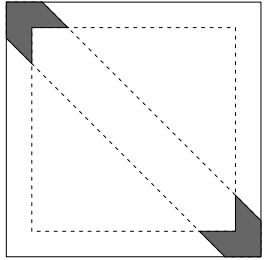
\includegraphics{carre.png}
\caption{La surface grisée est la surface dont on cherche le volume
(ici, \(d = 2\)). L'hyperplan définit dans le texte est ici donné par la
droite \(x_2 = 1 - x_1\).}
\end{figure}

\begin{enumerate}
\def\labelenumi{\arabic{enumi}.}
\item
  Justifier que le volume considéré grandit avec \(d\). \emph{On pourra
  justifier que le premier volume tende vers 1 quand
  \(d\rightarrow \infty\) et que le second se stabilise vers une valeur
  finie}. \emph{L'argument pour le premier volume est purement
  géométrique, l'argument pour le second peut se déduire du TCL}.
\item
  Ecrire le volume recherché sous forme d'une intégrale. En déduire un
  estimateur Monte Carlo de ce volume.
\item
  Donner une estimation de ce volume pour \(\varepsilon = 0.1\) et
  \(d = 2, 5, 10, 20\). Vous choisirez vous même l'effort de Monte
  Carlo, en justifiant ce choix. Donnez l'incertitude associée à votre
  estimation.
\item
  À l'aide de la fonction \texttt{hcubature} du package
  \texttt{cubature}, donnez une valeur du volume obtenue par
  approximation numérique pour les mêmes valeurs de \(d\).
\item
  Comparez les résultats et commentez.
\end{enumerate}

\hypertarget{cas-des-uxe9vuxe8nements-rares}{%
\section{Cas des évènements
rares}\label{cas-des-uxe9vuxe8nements-rares}}

On se propose d'étudier l'erreur relative de l'estimateur de Monte Carlo
de la probabilité \(p\) d'un événement \(E\) (\(0 < p \leq 1\)), en
fonction de la valeur de \(p\).

On se place dans le cas où pour estimer \(p\), on simule \(n\) variables
aléatoires indépendantes \(X_1,\dots, X_n\) de loi de Bernouilli de
paramètre \(p\).

L'estimateur de Monte Carlo de \(p\) est donné par
\[\hat{p} = \bar{X}_n = \frac{1}{n}\sum_{i = 1}^n X_i\] On s'intéresse à
l'erreur relative de \(\hat{p}\), à savoir la quantité:
\[\Delta_p = \frac{\hat{p} - p}{p}\]

\begin{enumerate}
\def\labelenumi{\arabic{enumi}.}
\tightlist
\item
  Calculer la variance de \(\Delta_p\).
\item
  Pour \(0 < \alpha < 1\), exprimer \(\mathbb{P}(|\Delta_p| > \alpha)\)
  exactement en fonction de la loi d'une variable aléatoire binomiale de
  paramètres \((n, p)\). Que pouvez vous conjecturer sur cette
  probabilité quand \(p\) devient petit?
\item
  En utilisant le théorème central limite, donner une expression
  asymptotique de cette probabilité basée sur la fonction de répartition
  de la loi normale centrée réduite.
\end{enumerate}

\hypertarget{attention-uxe0-la-dimension}{%
\subsection{Attention à la
dimension!}\label{attention-uxe0-la-dimension}}

\begin{enumerate}
\def\labelenumi{\arabic{enumi}.}
\setcounter{enumi}{3}
\item
  On peut montrer que le volume d'une sphère de rayon 1 en dimension
  \(d\geq 2\) est donné par la fonction:
  \[V(d) = \frac{\pi^{d / 2}}{\Gamma(\frac{d}{2} + 1)}\] où, pour
  \(z>0\) \[\Gamma(z) = \int_0^\infty t^{z-1} e^{-t} d t\] On se propose
  d'estimer la valeur de \(\pi\) en tirant, en dimension \(d\), une
  \(U\) variable uniforme dans l'hypercube \([-1, 1]^d\). On pose alors
  \(X = \mathbf{1}_{\parallel U \parallel^2 \leq 1}\), sur un
  échantillon de taille \(n = 10000\).

  \begin{enumerate}
  \def\labelenumii{\alph{enumii}.}
  \tightlist
  \item
    Quelle est la valeur de \(p\), le paramètre de la loi de Bernouilli
    de \(X\)?
  \item
    Donner alors l'estimateur de \(\pi\) en fonction de l'estimateur de
    \(p\).
  \item
    Discutez la qualité de l'estimateur quand \(d\) grandit. Vous
    pourrez vous aidez de R pour voir le comportement de la fonction
    \(V_d\) (en pourra utiliser la fonction \texttt{gamma} dans R).
  \end{enumerate}
\end{enumerate}

\hypertarget{duxe9tection-daggruxe9gats-dans-une-suxe9rie-temporelle}{%
\section{Détection d'aggrégats dans une série
temporelle}\label{duxe9tection-daggruxe9gats-dans-une-suxe9rie-temporelle}}

\hypertarget{pruxe9sentation-du-probluxe8me}{%
\subsection{Présentation du
problème}\label{pruxe9sentation-du-probluxe8me}}

On s'intéresse à une série temporelle à valeurs dans \(\mathbb{R}\).
Ainsi, les données consistent en un vecteur
\(X_{1:n} = (X_1,\dots X_n)\) de valeurs ordonnées dans le temps.

La question est la suivante: \emph{Existe-t-il une fenêtre temporelle de
valeurs anormalement élevées?}.

Pour cela, on se propose de faire le test

\begin{itemize}
\tightlist
\item
  \(H_0\): Les variables aléatoires \(X_1,\dots, X_n\) sont
  indépendantes et identiquement distribuées.
\item
  \(H_1\): Il existe une fenêtre temporelle où les valeurs de la série
  sont plus importantes.
\end{itemize}

Pour tester cette hypothèse, pour une série temporelle
\(X_{1:n} = (X_1,\dots, X_n)\), on va définir une statistique de test
\(T(X_{1:n})\).

Pour l'échantillon aléatoire \(X_1,\dots X_n\), on note \(R_k\) le rang
de \(X_k\) parmi les valeurs de l'échantillon (il est égal à 1 si
\(X_k\) est la valeur la plus faible, à \(n\) si \(X_k\) est la valeur
la plus élevée). Comme on considère des variables aléatoires continues,
on considère dans la suite que deux rangs ne peuvent pas être égaux.
\textbf{Vous remarquerez que l'hypothèse H0 ne fait pas d'hypothèse sur
la distribution des valeurs observées, en effet, H0 fait une hypothèse
sur la distribution jointe des rangs}.

\begin{enumerate}
\def\labelenumi{\arabic{enumi}.}
\tightlist
\item
  Justifier que, sous \(H_0\), la loi de \(R_k\) est une loi uniforme
  discrète sur \(\left\lbrace 1,\dots,n\right\rbrace\). Quelle est la
  loi de \(R_k\) sachant \(R_\ell\) (\(\ell\neq k\))?
\end{enumerate}

Pour tout couple \((i, j)\) tel que \(1 \leq i\leq j\leq n\) on
considère la variable aléatoire suivante:

\[S(i, j) = \sum_{k = i}^j R_k.\]

\begin{enumerate}
\def\labelenumi{\arabic{enumi}.}
\setcounter{enumi}{1}
\item
  Que représente cette variable aléatoire? Dans quel cas prendra t'elle
  des grandes valeurs?
\item
  Montrer que, sous \(H_0\),
  \(m_{ij} := \mathbb{E}[S(i,j)] = \frac{1}{2}(n+1)(j-i+1)\) pour tout
  couple \((i,j)\).
\item
  Calculer, sous \(H_0\),
  \(v_{ij} := \mathbb{V}[S(i,j)] = \frac{1}{12}(n+1)(j-i+1)(n-j+i-1)\)
  pour tout couple \((i,j)\).
\end{enumerate}

On définit maintenant la variable aléatoire centrée et réduite, pour
tout couple d'entiers \((i, j)\) tel que \(1 \leq i\leq j\leq n\).
\[T(i, j) = \left\lbrace \begin{array}{lr}
0&\text{ si } i = 1 \text{ et } j = n\\
\frac{S(i, j) - m_{ij}}{\sqrt{v_{ij}}} & \text{ sinon.} 
\end{array}
\right.\]

Notre statistique de test \(T_n(X_{1:n})\) sera donc donnée par
\begin{equation}
\label{eq:stat:T}
T_n(X_{1:n}) = \underset{1 \leq i\leq j\leq n}{\text{max}} T(i, j).
\end{equation}

\hypertarget{principe-du-test-et-prise-de-duxe9cision-par-muxe9thode-de-monte-carlo.}{%
\subsection{Principe du test et prise de décision par méthode de Monte
Carlo.}\label{principe-du-test-et-prise-de-duxe9cision-par-muxe9thode-de-monte-carlo.}}

Le principe du test est le suivant: pour un échantillon observé
\(\mathbf{x}\) un risque \(\alpha\), on rejette \(H_0\) si
\(T_n(\mathbf{x}) > t_{1 - \alpha}\) où \(t_{1 - \alpha}\) est le
quantile d'ordre \(\alpha\) de la loi de \(T_n(\mathbf{X})\). On
concluera que la fenêtre temporelle pour laquelle la statistique est
calculée (soit
\((i_{\text{max} },j_{\text{max}}) = \text{argmax}_{i,j}~T(i,j)\)) est
anormalement loin de 0 sous \(H_0\). On rejettera alors \(H_0\) pour
conclure a un aggrégat de valeurs élevées sur cette fenêtre.

\begin{enumerate}
\def\labelenumi{\arabic{enumi}.}
\setcounter{enumi}{4}
\item
  La loi de \(T_n\) sous \(H_0\) étant inconnue, on se propose
  d'approcher ses quantiles sous \(H_0\) par méthode de Monte Carlo.
  Donner un algorithme simple de simulation de \(T_n\) sous \(H_0\).
\item
  Proposer une méthode de Monte Carlo pour répondre à la question
  initiale à un risque \(\alpha\) fixé, pour n'importe quelle série
  temporelle observée \(x_{1:n}\).
\end{enumerate}

\hypertarget{impluxe9mentation-sous-r-pour-les-tempuxe9ratures-uxe0-hobart-tasmanie.}{%
\subsection{Implémentation sous R pour les températures à Hobart,
Tasmanie.}\label{impluxe9mentation-sous-r-pour-les-tempuxe9ratures-uxe0-hobart-tasmanie.}}

\begin{enumerate}
\def\labelenumi{\arabic{enumi}.}
\setcounter{enumi}{6}
\item
  Ecrire une fonction \texttt{get\_tn}, qui pour une série temporelle
  \(x_{1:n}\) donnée, calcule \(T_n(x_{1:n})\) et, si on le demande,
  renvoit les indices temporels de la fenêtre sur laquelle cette
  statistique est obtenue. Calculer cette statistique de test pour la
  série des températures à Hobart. On notera cette valeur \(t^*\)
\item
  Ecrire une fonction \texttt{get\_h0\_sample} qui, pour un entier \(n\)
  et un entier \(M\) permet d'obtenir \(M\) réalisations de \(T_n\) sous
  \(H_0\).
\item
  Simuler un \(M\) échantillon de \(T_n\) sous \(H_0\) pour une valeur
  de \(n\) correspondant à celles des données d'Hobart. Vous prendrez
  \(M = 5000\). Représenter l'estimation obtenue de
  \(\mathbb{P}(T_n > t^*)\) ainsi que son intervalle de confiance
  asymptotique à 95\%.
\item
  Répondre à la question initiale sur les températures à Hobart
\end{enumerate}


\end{document}
